% !TeX root = ../tfg.tex
% !TeX encoding = utf8

\chapter{Redes neuronales prealimentadas}\label{chap:ann}

Las redes neuronales son un tipo de modelos del aprendizaje automático. El aprendizaje automático puede definirse como
el conjunto de métodos computacionales que utilizan la experiencia para realizar predicciones precisas y tomar 
decisiones. Lo que denominamos experiencia se refiere a información previa accesible al modelo, que normalmente suele 
corresponderse con conjuntos de datos de los que queremos extraer un cierto conocimiento 
\cite{mohri_rostamizadeh_talwalkar_2018}. 

\vspace{10pt}
Específicamente, el aprendizaje automático es el conjunto de algoritmos y modelos estadísticos que permiten realizar 
tareas computacionales complejas sin instrucciones explícitas. En lugar de ser programados, estos modelos pueden 
realizar tareas específicas mediante un proceso de entrenamiento a partir de datos, lo que les permite reconocer 
patrones y tomar decisiones basadas en nuevos datos. Los modelos que vamos a utilizar en este trabajo son capaces de 
solucionar los siguientes tipos de problemas:

\begin{itemize}
    \item \textbf{Clasificación}: La clasificación es un tipo de problema que que consiste en asignar una categoría a cada elemento. Por ejemplo, asignar conjuntos de datos meteorológicos a las categorías nublado, soleado o lluvia.
    \item \textbf{Regresión}: La regresión es el problema de predecir un valor continuo para cada elemento. Ejemplos
    de regresión pueden ser predecir el valor de las acciones de una empresa a partir de sus datos económicos o 
    calcular la esperanza de vida de un individuo a partir de datos médicos y de costumbres.
\end{itemize}

El primer trabajo conocido que responde a la idea de crear modelos capaces de aprender simulando el comportamiento de
las neuronas es el de Warren McCulloch y Walter Pitts en 1943. En él, se introduce el concepto de red neuronal 
artificial y algunas características como la actividad binaria de una neurona, además de la distinción en lo que
actualmente se conocen como neuronas de entrada y de salida \cite{mcculloh-pitts}. A raíz de ese trabajo y posteriores,
el concepto de red neuronal se ha extendido a multitud de distintos modelos, todos basados en la idea de combinar
unidades de procesamiento, denominadas \textit{neuronas}, para realizar múltiples tareas computacionales. 

\vspace{10pt}
Dentro de las redes neuronales, podemos encontrar modelos muy simples, como el del perceptrón, descrito en 1958 por 
Frank Rossenblatt en 
\textit{The Perceptron: A Probabilistic Model for Information Storage and Organization in the Brain}, útil para 
resolver problemas linealmente separables; hasta modelos mucho más complejos, como las redes generativas adversativas 
(GANs en inglés), descritas por Ian Goodfellow y otros en \textit{Generative Adversarial Networks} y utilizadas para la 
generación de imágenes o música, por ejemplo \textit{museGAN}, una red neuronal capaz de construir piezas de música con 
cuatro pistas de audio \cite{dong_hsiao_yang_yang_2018}.

\vspace{10pt}
Las redes neuronales utilizan conjuntos de datos para su aprendizaje, y para ellos definimos los siguientes conceptos, 
para los cuales tomaremos como ejemplo ilustrativo el problema de clasificar flores en varias especies a partir de 
información acerca de las mismas:

\begin{itemize}
    \item \textbf{Ejemplos}: Conjunto de datos utilizado para el aprendizaje. En nuestro caso, el conjunto de 
    información acerca de las flores.
    \item \textbf{Características}: Conjunto de atributos asociados a un ejemplo. En el caso de las flores, estos
    pueden ser el tamaño de los pétalos, su color, \dots
    \item \textbf{Etiquetas}: Valores o categorías asignadas a los ejemplos. En problemas de clasificación son la
    categoría de ese ejemplo, como sería la especie de flor en nuestro conjunto, mientras que en problemas de regresión
    es un valor real.
    \item \textbf{Conjunto de entrenamiento}: Subconjunto de los ejemplos que se utilizan para el ``entrenamiento'' de
    la red, es decir, el conjunto de datos que se utiliza para el aprendizaje del modelo.
    \item \textbf{Conjunto de test}: Subconjunto de los ejemplos utilizados para evaluar el rendimiento de la red. Este
    subconjunto debe ser disjunto con el conjunto de entrenamiento, para asegurar una evaluación real del 
    funcionamiento.
\end{itemize}

\vspace{10pt}
La herramienta desarrollada en este trabajo se centra en las redes neuronales prealimentadas con una capa oculta. Es 
para este tipo de redes para las que se ha automatizado la distribución del proceso de aprendizaje. En este capítulo, 
definiremos este tipo de redes neuronales, su uso y la implementación de las mismas en la librería de Scala creada para
el posterior intérprete.

% -------------------------------------------------------------------------------------------------------------------
\section{Definición y componentes}

\begin{figure}[htbp!]
    \centering
    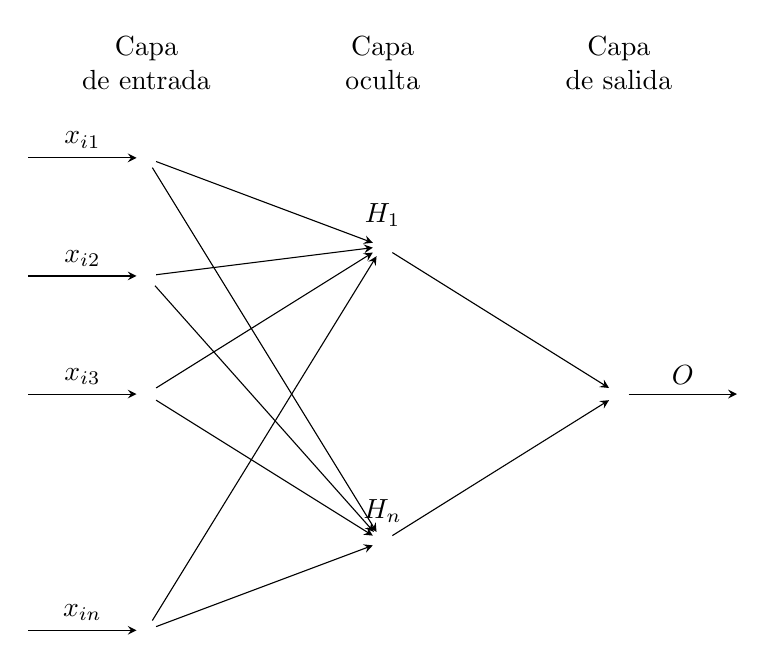
\begin{tikzpicture}[x=1.5cm, y=1.5cm, >=stealth]

\foreach \m/\l [count=\y] in {1,2,3,missing,4}
  \node [every neuron/.try, neuron \m/.try] (input-\m) at (0,2.5-\y) {};

\foreach \m [count=\y] in {1,missing,2}
  \node [every neuron/.try, neuron \m/.try ] (hidden-\m) at (2,2-\y*1.25) {};

\foreach \m [count=\y] in {1}
  \node [every neuron/.try, neuron \m/.try ] (output-\m) at (4,0.5-\y) {};

\foreach \l [count=\i] in {1,2,3,n}
  \draw [<-] (input-\i) -- ++(-1,0)
    node [above, midway] {$x_{i\l}$};

\foreach \l [count=\i] in {1,n}
  \node [above] at (hidden-\i.north) {$H_\l$};

\foreach \l [count=\i] in {1}
  \draw [->] (output-\i) -- ++(1,0)
    node [above, midway] {$O$};

\foreach \i in {1,...,4}
  \foreach \j in {1,...,2}
    \draw [->] (input-\i) -- (hidden-\j);

\foreach \i in {1,...,2}
  \foreach \j in {1}
    \draw [->] (hidden-\i) -- (output-\j);

\foreach \l [count=\x from 0] in {de entrada, oculta, de salida}
  \node [align=center, above] at (\x*2,2) {Capa \\ \l};

\end{tikzpicture}
    \caption{Red neuronal prealimentada con una capa oculta}
    \label{fig:mlp}
\end{figure}

Una red neuronal prealimentada, conocida históricamente también como perceptrón multicapa, es un sistema de componentes 
de procesamiento de varias capas, como el descrito en la figura \ref{fig:mlp}. La primera capa de esta red se le llama 
capa de entrada y es la que recibe los datos, todas las intermedias son denominadas capas ocultas y la última es 
denominada capa de salida. Gracias a estas capas ocultas, la red puede extraer resultados más complejos a partir de los 
datos. En un sentido poco formal, podemos decir que mediante este aumento de dimensiones de interacción entre neuronas, 
la red obtiene una perspectiva ``global'' \cite{haykin_1999}. 

\vspace{10pt}
Las redes neuronales prealimentadas son capaces de 
resolver problemas de aprendizaje automático mediante \textit{aprendizaje supervisado}. En este tipo de aprendizaje, el 
modelo recibe como conjunto de entrenamiento datos etiquetados previamente y realiza predicciones de las etiquetas de 
los ejemplos \cite{mohri_rostamizadeh_talwalkar_2018}.

\vspace{10pt}
En las redes neuronales prealimentadas, cada neurona está conectada con todas las neuronas de las capas vecinas, y un 
peso es asignado a cada una de esas conexiones. Estas neuronas nunca están conectadas a otras neuronas de su misma capa
ni a neuronas de capas que no son adyacentes. Además, las conexiones a la capa anterior son siempre de entrada, funcionando como conexiones de salida las que se conectan con la siguiente capa. Los datos de entrada son suministrados 
a la capa de entrada, y son procesados de manera ascendente en las capas hasta llegar a la salida \cite{Yagawa2021}. Es 
por este camino que toman los datos (de izquierda a derecha y en una única dirección) por lo que se las denomina redes 
neuronales prealimentadas, \textit{feed-foward neural networks} en inglés. 

% -------------------------------------------------------------------------------------------------------------------
\subsection{Neuronas}

Veamos ahora de qué se compone una neurona y cuál es su funcionamiento. Identificamos tres elementos básicos de las
neuronas de una red:
\begin{enumerate}
    \item Un conjunto de conexiones o \textit{sinapsis} con un peso asignado a cada una de ellas, es decir, para un
    valor de entrada de una conexión $x_j$ a una neurona $k$, ese valor es multiplicado por un peso $w_{kj}$.
    \item Una función de adición o \textit{combinador lineal} que realiza una suma ponderada de todos los valores de 
    entrada de la neurona, utilizando sus respectivos pesos. Para una neurona $k$, se describe esta función de la
    siguiente manera:
    \begin{equation}\label{eq:neurona}
        u_k(x)=\sum_{j=1}^mw_{kj}x_j+b_k
    \end{equation}
    donde
    \begin{description}
        \item[$m$] es el número de conexiones de entrada de la neurona.
        \item[$x=(x_1,\dots,x_m)$] son los valores de entrada.
        \item[$w_{k1},\dots,w_{km}$] son los pesos de las conexiones.
        \item[$b_k$] es un valor de sesgo para la neurona.
    \end{description}
    El valor de sesgo de la neurona es esencial, ya que sin él el hiperplano generado por la función incluye siempre el
    origen de coordenadas, limitando la variabilidad y la capacidad de aprendizaje de la neurona. Si añadimos una nueva 
    conexión, cuyo valor de entrada sea $x_0=1$ y su peso $w_{k0}=b_k$, podemos reescribir la ecuación anterior de la 
    siguiente manera:
    \begin{equation}
        v_k(x)=\sum_{j=0}^mw_{kj}x_j
    \end{equation}
    \item Una \textit{función de activación} $\varphi$ que acota la amplitud de la salida de la neurona. Esta 
    función transforma los valores de salida del combinador lineal a valores dentro de un intervalo mucho más 
    pequeño. Los intervalos más usuales suelen ser $[0,1]$ y $[-1,1]$. Para eliminar la linealidad de las redes, 
    normalmente se suelen utilizar como funciones de activación la función sigmoide y la tangente hiperbólica, que justamente acotan la salida de la neurona a los intervalos $[0,1]$ y $[-1,1]$, respectivamente. Estas funciones 
    tienen la siguiente expresión:
    \begin{equation}
        \text{sigmoide}(v)=\frac{1}{1+e^{-v}}\quad\quad\tanh(v)=\frac{e^v-e^{-v}}{e^v+e^{-v}}
    \end{equation}
    Al resultado de aplicar la función de activación a la neurona se le suele denotar como $\tilde{y}_k$.
\end{enumerate}

Un esquema de estas neuronas es el de la figura \ref{fig:neurona} \cite{haykin_1999}.

\begin{figure}[htbp!]
    \centering
    \begin{tikzpicture}[x=1.cm, y=1.5cm, >=stealth]

\foreach \m/\l [count=\y] in {1,2,3,missing,4}
  \node [every neuron/.try, neuron \m/.try, draw=none] (input-\m) at (0,2.5-\y) {};

\foreach \m [count=\y] in {1}
  \node [semi,shape border rotate=90] (output-\m) at (2,0.5-\y) {$\sum$};
  \node [semi,right=0cm of output-1,shape border rotate=270] (output-f) {$\varphi$};

\foreach \l [count=\i] in {1,2,3,j}
  \draw (input-\i) ++(0,0)
    node {$x_\l$};

\foreach \l [count=\i] in {f}
  \draw [->] (output-\l) -- ++(1,0)
    node [above, midway] {$\tilde{y}_k$};

\foreach \i in {1,...,4}
  \foreach \j in {1}
    \draw [->] (input-\i) -- (output-\j);
\end{tikzpicture}
    \caption{Esquema de una neurona}
    \label{fig:neurona}
\end{figure}

\vspace{10pt}
Existen ciertas particularidades para las neuronas de la capa de entrada y las de la capa de salida. Las neuronas de la
capa de entrada tienen únicamente una conexión de entrada, que se corresponde al valor de una de las características de
los ejemplos. Tampoco se le suele asignar un peso a este valor de entrada, y como función de activación se utiliza la
función identidad \cite{Yagawa2021}. Para las neuronas de la capa de salida, si se trata de un problema de regresión,
suele también utilizarse la función de identidad como función de activación, puesto que usualmente el valor a predecir
no suele estar acotado al intervalo unidad. En los problemas de clasificación, se utiliza una función umbral para
asignar la categoría al resultado de la suma ponderada \cite{mlp}. Esta función tiene la siguiente expresión:
\begin{equation}
    f(v)=\begin{cases}
        1 & \text{si}\quad v>0.5 \\
        -1 & \text{en cualquier otro caso} 
    \end{cases}
\end{equation}


% -------------------------------------------------------------------------------------------------------------------
\subsection{Predicciones, medidas de rendimiento y algoritmo de aprendizaje}

\subsubsection*{Predicciones}

El objetivo de una red prealimentada es realizar predicciones a partir de un conjunto de datos de entrada. Para 
realizar una de estas predicciones, se utiliza la \textit{propagación hacia delante}, que no es más que, a partir de
los datos de entrada, calcular los valores de salida de las neuronas capa a capa hasta llegar a la capa final. 
Supongamos que tenemos una red con dos neuronas de entrada, tres neuronas en una capa oculta y una neurona en la capa
de salida, y se trata de una red que pretende clasificar. Sea $x=(x_1,x_2)$ un ejemplo, y denotando con un superíndice 
la capa de la neurona y con un subíndice la neurona de esa capa, podemos predecir su etiqueta de la siguiente manera:
\begin{enumerate}
    \item Para la capa de entrada, su salida serán los mismos datos de entrada. Por tanto, si denotamos la salida de esta capa como $x^{(1)}$, $x^{(1)}_1=x_1$ y $x^{(1)}_2=x_1$.
    \item Para la capa oculta, la salida de cada neurona $k$ la calculamos como:
    \begin{equation}
        x^{(2)}_k=\varphi(\sum_{i=0}^2w^{(2)}_{kj}x^{(1)}_i)
    \end{equation}
    \item Finalmente, la predicción de la red sera, utilizando la capa de salida y denotando la función umbral por $f$:
    \begin{equation}
        \tilde{y}=f(\varphi(\sum_{i=0}^3w^{(3)}_jx^{(2)}_i))
    \end{equation}
\end{enumerate}

Podemos ver, de esta manera, que toda red neuronal puede ser representada como una composición de funciones donde capa
etapa está anidada en la siguiente etapa. La propagación hacia delante es un paso indispensable para el posterior 
cálculo de las medidas de rendimiento, que a su vez son utilizadas por los algoritmos de aprendizaje para mejorar la 
calidad de las predicciones\cite{mlp}. 

\subsubsection*{Medidas de rendimiento}

Para determinar el rendimiento de la red, se utilizan medidas que llamaremos \textit{funciones de coste}, 
\textit{funciones de pérdida} o \textit{funciones objetivo}. Convencionalmente, se llama \textit{funciones de pérdida} 
a la medida de error de un ejemplo de entrenamiento, \textit{función de coste} a la agregación de las funciones de 
pérdida del conjunto de entrenamiento completo y \textit{función objetivo} a la medida general del error en la red 
\cite{mlp}. 

\vspace{10pt}
Las funciones de coste son utilizadas por los algoritmos de aprendizaje para conocer la ``bondad'' de las predicciones 
durante el entrenamiento. La función de coste más usual es el error cuadrático medio, que tiene la siguiente expresión:
\begin{equation}
    \text{MSE}=\frac 1n\sum_{i=1}^n(y_i-\tilde{y}_i)^2
\end{equation}
donde $n$ es el conjunto de ejemplos de entrenamiento, $y_i$ las etiquetas de cada ejemplo y $\title{y}_i$ las 
predicciones de la red de cada ejemplo.

\vspace{10pt}
Para los problemas de clasificación, una de las maneras más exhaustivas de representar el rendimiento de la red es la
matriz de confusión. Se trata de una matriz $2\times 2$, donde las filas se corresponden a las posibles categorías y
las columnas a las categorías predichas. De esta manera, los valores estimados correctamente por el modelo son los de 
la diagonal principal, mientras que las predicciones erróneas se corresponden a la diagonal secundaria 
\cite{muller_guido_2017}. Si definimos las categorías como ``positiva'' y ``negativa'', la matriz de confusión se puede 
representar como la figura \ref{fig:conf-mat}. 

\begin{figure}[htb!]
    \centering
    \begin{tikzpicture}[
box/.style={draw,rectangle,minimum size=3cm,text width=2.5cm,align=left}]
\matrix (conmat) [row sep=.1cm,column sep=.1cm] {
\node (tpos) [box,
    label=left:\( \mathbf{p} \),
    label=above:\( \mathbf{\tilde{p}} \),
    ] {Verdaderos \\ positivos \\ (VP)};
&
\node (fneg) [box,
    label=above:\( \mathbf{\tilde{n}} \),
    label=above right:\textbf{total},
    label=right:\( \mathrm{P} \)] {Falsos \\ negativos \\ (FN)};
\\
\node (fpos) [box,
    label=left:\( \mathbf{n} \),
    label=below left:\textbf{total},
    label=below:\( \mathrm{\tilde{P}} \)] {Falsos \\ positivos \\ (FP)};
&
\node (tneg) [box,
    label=right:\( \mathrm{N} \),
    label=below:\( \mathrm{\tilde{N}} \)] {Verdaderos \\ negativos \\ (VN)};
\\
};
\node  [rotate=90,left=.05cm of conmat,anchor=center,text width=1.5cm,align=center] {\textbf{Etiquetas \\ reales}};
\node [above=.05cm of conmat] {\textbf{Etiquetas predichas}};
\end{tikzpicture}
    \caption{Matriz de confusión}
    \label{fig:conf-mat}
\end{figure}

\vspace{10pt}
Podemos abreviar los elementos de la matriz por sus iniciales. Notaremos VP a los verdaderos positivos, FP a los falsos
positivos, VN a los verdaderos negativos y FN a los falsos negativos. A partir de la matriz de confusión, podemos 
definir medidas concretas que resumen la información proporcionada por la misma:

\vspace{10pt}\textbf{\textit{Exactitud}}: La exactitud o \textit{accuracy} representa 
el porcentaje de predicciones correctas realizadas por el modelo. Se calcula de la 
siguiente manera.
\begin{equation}
    \text{\textit{Exactitud}}=\frac{VP+VN}{VP+VN+FP+FN}
    =\frac{VP+VN}{P+N}=\frac{VP+VN}{\tilde{P}+\tilde{N}}
\end{equation}

\vspace{10pt}\textbf{\textit{Precisión}}: La \textit{precision}, en castellano precisión, mide la relación entre los
verdaderos positivos y el total de positivos, y tiene la siguiente expresión:
\begin{equation}
    \text{\textit{Precisión}}=\frac{VP}{VP+FP}=\frac{VP}{\tilde{P}}
\end{equation}
Esta medida suele utilizarse cuando es importante para el modelo minimizar el número de falsos positivos. Se le puede
denominar también como \textit{valor predictivo positivo} (\textit{positive predictive value} en inglés).

\vspace{10pt}\textbf{\textit{Sensibilidad}}: La sensibilidad o \textit{recall} es una medida que permite calcular el 
porcentaje de verdaderos positivos sobre el total de predicciones positivas. Se calcula como:
\begin{equation}
    \text{\textit{Sensibilidad}}=\frac{VP}{VP+FN}=\frac{VP}{P}
\end{equation}
A diferencia de la precisión, esta medida es importante cuando queremos evitar los falsos negativos. Es conocida también
como \textit{ratio de verdaderos positivos}.

\vspace{10pt}\textbf{\textit{$f_1$-score}}: El \textit{$f_1$-score} o puntuación $f_1$ es una medida que combina la
precisión y la sensibilidad. En particular, se trata de la media armónica de esas dos medidas:
\begin{equation}
    f_1=\frac{\text{\textit{Sensibilidad}}
\cdot\text{\textit{Precisión}}}{\text{\textit{Sensibilidad}}+\text{\textit{Precisión}}}
\end{equation}
La puntuación $f_1$ suele ser utilizada para medir la bondad de la red cuando el conjunto de datos sobre el que estamos
trabajando posee un número desequilibrado de ejemplos de cada categoría \cite{muller_guido_2017}.

\subsubsection*{Algoritmo de aprendizaje}

Para poder realizar predicciones adecuadas, una red neuronal necesita un algoritmo de aprendizaje que modifique los
pesos de sus neuronas a partir de la función de coste utilizada. Un algoritmo de aprendizaje se compone de las 
siguientes etapas:
\begin{enumerate}
    \item \textbf{Inicialización}: En este paso, todos los pesos de la red son inicializados con valores aleatorios.
    Debido a esta aleatoriedad, normalmente se realizan varios entrenamientos del modelo y se toma el que de mejores
    resultados.
    \item \textbf{Propagación hacia delante}: Se realiza la predicción de ejemplos de entrenamiento mediante la
    propagación hacia delante, cuyo funcionamiento hemos descrito.
    \item \textbf{Propagación hacia atrás o retropropagación}: Utilizando las predicciones del paso anterior, y 
    mediante el uso de una función de costo, se modifican los valores de los pesos y sesgo en orden descendente. Después, se pasa al paso 2 de nuevo y así de forma repetitiva hasta que se cumple una condición de salida, como 
    puede ser el número de veces que se utiliza el conjunto de datos completo (épocas), el número total de veces que se ejecuta la retropropagación (nº de iteraciones), valor umbral de error, \dots El algoritmo tradicionalmente 
    utilizado para esta fase es el descenso de gradiente. Este método modifica los pesos de la red de la siguiente 
    manera:
    \begin{gather}
        \Delta w^{(p)}_{ji}=-\frac{\partial E}{\partial w^{(p)}_{ji}} \\
        w^{(p)}_{ji}=w^{(p)}_{ji}+\alpha\cdot\Delta w^{(p)}_{ji}
    \end{gather}
    donde $\Delta w^{(p)}_{ji}$ es la modificación del peso $i$-ésimo de la neurona $j$ de la capa $p$, $E$ es la
    función de costo y $\alpha$ es un parámetro, llamado ratio de aprendizaje, que escala la modificación de los
    pesos \cite{Yagawa2021}.\\
    Existen multitud de algoritmos aparte del descenso de gradiente, optimizados para cierto tipo de redes, conjuntos
    de datos o recursos computacionales. En este trabajo, se utiliza para las redes el algoritmo de optimización por
    enjambre de partículas, definido más adelante.
\end{enumerate}

% -------------------------------------------------------------------------------------------------------------------
\section{Aproximadores universales}

Una pregunta que puede surgir acerca de las redes neuronales prealimentadas es, ¿son capaces estos modelos de resolver
o aproximarse a la solución de los problemas para los cuales han sido creadas? Todo problema de aprendizaje automático
lo podemos ver como la búsqueda de una función tal que, tomando como entrada la información de la que disponemos, 
sea capaz de dar la solución o predicción correcta siempre. Por ejemplo, que sea capaz de determinar el diagnóstico
correcto siempre a partir de datos médicos. A esta función se la suele denominar \textit{función objetivo}. 

\vspace{10pt}
En 1989 Kurt Hornik, Maxwell Stinchcombe y Halbert White demostraron que toda red neuronal prealimentada es un 
aproximador universal. En particular, demostraron que:
\begin{quote}
    Las redes neuronales prealimentadas con al menos una capa oculta usando una función de activación sigmoidea 
    arbitraria son capaces de aproximar cualquier función boreliana medible que vaya de un espacio de dimensión finita 
    a otro con el grado de precisión que se desee, siempre que haya suficientes capas ocultas. En este sentido, las 
    redes neuronales prealimentadas son aproximadores universales. \cite{hornik_1989}
\end{quote}
Poco después, en 1991, Hornik demostró que no es necesario que la función de activación sea sigmoidea para considerar 
estas redes como aproximadores universales. Veamos unas pinceladas de este trabajo, puesto que para mostrar las 
pruebas completas es necesario utilizar conceptos avanzados del análisis funcional. Para ello, vamos a trabajar con 
una red neuronal prealimentada con una única capa oculta y una única neurona de salida, que es justamente el tipo de 
neuronas implementadas en este trabajo. Entonces, el conjunto de funciones que implementan esas redes, con $n$ neuronas 
ocultas es
\begin{equation}
    \mathfrak{R}_k^{(n)}(\varphi)=\Big\{h:\mathbb{R}^k\to\mathbb{R}\mid h(x)=f(\sum_{j=1}^n\varphi(w_j^Tx+b_j))\Big\}
\end{equation}
donde $\varphi$ es la función de activación común para todas las neuronas y $T$ denota la transposición de forma que si
$w_j=(w_{j1},\dots,w_{jk})$ y $x=(x_1,\dots,x_k)$, $w_j^Tx$ denota el producto escalar \cite{hornik_1991}. Podemos ver 
que la notación $w_j^Tx+b_j$ es equivalente a la de la ecuación \eqref{eq:neurona}. El conjunto de todas las funciones
implementadas por este tipo de red con un número arbitrariamente grande de neuronas ocultas es entonces:
\begin{equation}
    \mathfrak{R}_k(\varphi)=\bigcup_{n=1}^\infty\mathfrak{R}_k^{(n)}(\varphi)
\end{equation}

Definimos ahora el espacio de funciones en el cual se encuentran nuestros modelos. Sea $\mu$ una medida, para 
$1\leq p<\infty$ definimos la norma:
\begin{equation}
    \|f\|_{p,\mu}=\Big[\int_{\mathbb{R}^k}|f(x)|^pd\mu(x)\Big]^{\frac 1p}
\end{equation}

\begin{definicion}$L^p(\mu)$ es el espacio de funciones $f$ tal que $\|f\|_{p,\mu}<\infty$. Diremos que 
$S\subset L^p(\mu)$ es \textit{denso} en $L^p(\mu)$ si para cualquier $f\in L^p(\mu)$ y $\epsilon>0$, existe una función
$g\in S$ tal que $\|f-g\|_{p,\mu}<\epsilon$.
\end{definicion}

Con estas definiciones, llegamos a un primer resultado:

\begin{teorema}Si $\varphi$ es no constante y no acotada, entonces $\mathfrak{R}_k(\varphi)$ es denso en $L^p(\mu)$ 
para todas las medidas $\mu$ finitas en $\mathbb{R}^k$ \cite{hornik_1991}.
\end{teorema}

Tenemos entonces que toda red neuronal prealimentada es densa en $L^p(\mu)$, es decir, podemos aproximar cualquier
función de $L^p(\mu)$ mediante una red neuronal. Si ahora definimos, para $1\leq p<\infty$, la norma
\begin{equation}
    \|f\|_p=\Big[\int_{\mathbb{R}^k}|f(x)|^pdx\Big]^{\frac 1p}
\end{equation}
y denotamos $C(X)$ como el espacio de todas las funciones $f$ continuas en $X\subseteq\mathbb{R}^k$, entonces 
$S\subset C(X)$ es \textit{denso} en $C(X)$ si para cualquier $f\in C(X)$ y $\epsilon>0$, existe una función $g\in S$ 
tal que $\|f-g\|_p<\epsilon$. Podemos ahora dar un resultado equivalente al anterior pero para funciones continuas:

\begin{teorema}Si $\varphi$ es no constante y no acotada, entonces $\mathfrak{R}_k(\varphi)$ es denso en $C(X)$
para todos los subconjuntos compactos $X$ de $\mathbb{R}^k$ \cite{hornik_1991}.
\end{teorema}

Veamos ahora que podemos tomar $\varphi$ acotada y llegar a los mismos resultados. Para ello, vamos a definir algunos
conceptos. En primer lugar sea una $k$-tupla $\alpha=(\alpha_1,\dots,\alpha_k)$ de enteros no negativos, denominamos
\textit{orden} de $\alpha$ a $|\alpha|=\alpha_1+\cdots +\alpha_k$ y, para una función $f$ de $\mathbb{R}^k$, escribimos
su correspondiente derivada parcial como:
\begin{equation}
    D^\alpha f(x)=\frac{\partial^{\alpha_1+\cdots+\alpha_n}f}{\partial x_1^{\alpha_1}\cdots\partial x_k^{\alpha_k}}(x)
\end{equation}
Definimos ahora $C^m(\mathbb{R}^k)$ como el espacio de todas las funciones $f$ que, junto con sus derivadas parciales 
$D^\alpha f$ de orden $|\alpha|\leq m$, son continuas en $\mathbb{R}^k$. Definimos para $f\in C^m(\mathbb{R}^k)$ la
norma:
\begin{equation}
    \|f\|_{m}:=\max_{|\alpha|\leq m}\sup_{x\in\mathbb{R}^k}|D^\alpha f(x)|
\end{equation}
Diremos que $S\subset C^m(\mathbb{R}^k)$ es \textit{uniformemente $m$-denso sobre compactos} en $C^m(\mathbb{R}^k)$ si
para toda $f\in C^m(\mathbb{R}^k)$ y para todo $\epsilon>0$, existe una función $g\in S$ tal que $\|f-g\|_m<\epsilon$
\cite{hornik_1991}.

\vspace{10pt}
Ahora, sea $f\in  C^m(\mathbb{R}^k)$, $\mu$ una medida finita en $\mathbb{R}^k$ y $1\leq p<\infty$, definimos la norma
\begin{equation}
    \|f\|_{m,p}:=\Big[\sum_{|\alpha|\leq m}\int_{\mathbb{R}^k}|D^\alpha f|^pd\mu\Big]^{\frac 1p}
\end{equation}
y el espacio $C^{m,p}(\mu)$ como
\begin{equation}
    C^{m,p}(\mu)=\{f\in C^m(\mathbb{R}^k)\mid \|f\|_{m,p}<\infty\}
\end{equation}
Podemos ver que $C^{m,p}(\mu)=C^m(\mathbb{R}^k)$ si $\mu$ tiene soporte compacto. Diremos que $S$ es \textit{denso} en
$C^{m,p}(\mu)$ si para toda $f\in C^m(\mathbb{R}^k)$ y para todo $\epsilon>0$, existe una función $g\in S$ tal que
$\|f-g\|_{m,p}<\epsilon$ \cite{hornik_1991}. Tenemos, utilizando estas definiciones, los siguientes resultados:

\begin{teorema}Si $\varphi\in C^m(\mathbb{R}^k)$ es no constante y acotada, entonces $\mathfrak{R}_k(\varphi)$ es
uniformemente $m$-denso sobre compactos en $C^m(\mathbb{R}^k)$ y denso en $C^{m,p}(\mu)$ para todas las medidas finitas
de $\mathbb{R}^k$ con soporte compacto \cite{hornik_1991}.
\end{teorema}

Este resultado proporciona la justificación del uso de, por ejemplo, la tangente hiperbólica como función de activación.
Puesto que $\tanh\in C^\infty(\mathbb{R})$, entonces podemos resolver cualquier problema de aprendizaje cuya función
objetivo pertenezca a $C^m(\mathbb{R}^k)$.

\begin{teorema}Si $\varphi\in C^m(\mathbb{R}^k)$ es no constante y todas sus derivadas hasta orden $m$ son acotadas,
entonces $\mathfrak{R}_k(\varphi)$ es denso en $C^{m,p}(\mu)$ para todas las medidas finitas de $\mathbb{R}^k$ con 
soporte compacto \cite{hornik_1991}.
\end{teorema}

De esta manera, es fácil observar que las redes neuronales prealimentadas con al menos una capa oculta son, bajo 
condiciones muy generales sobre la función de activación de las neuronas ocultas, aproximadores universales, siempre y 
cuando la red tenga un número suficientemente grande de neuronas ocultas. Es importante notar que estos resultados no 
dan ninguna indicación constructiva, es decir, no proporcionan ninguna información acerca del número de capas ocultas, 
el número de neuronas ocultas o la función $\varphi$ más indicada para la aproximación \cite{hornik_1991}. Es por ello 
que, aunque tengamos la certeza de poder obtener un modelo que se aproxime casi a la perfección a la solución del 
problema, es necesario y recomendable realizar pruebas sobre los modelos modificando sus parámetros (número de neuronas 
de la capa oculta, iteraciones en el proceso de aprendizaje, \dots) para intentar encontrar ese teórico que aproxima la solución.

% -------------------------------------------------------------------------------------------------------------------
\section{Implementación}

Para construir las redes neuronales prealimentadas con una única capa oculta utilizadas en la herramienta, se ha 
utilizado una \textit{interfaz} de Scala (\texttt{trait}), que contiene la estructura común para tanto los 
clasificadores como los regresores. El código de esta interfaz se encuentra en el apéndice \ref{ap:estructura_ann},
así como el de las clases específicas. Este esqueleto para redes neuronales contiene:

\subsubsection*{Variables}
\begin{itemize}
    \item El número de neuronas de entrada y ocultas.
    \item Los conjuntos de ejemplos para entrenamiento y para test.
    \item Los pesos de la red.
    \item El objeto que calcula el error cuadrático medio de la red.
    \item El objeto que realiza la propagación hacia delante de la red.
    \item El objeto que contiene el algoritmo de aprendizaje de la red.
\end{itemize}
\subsubsection*{Métodos}
\begin{itemize}
    \item Una función para proporcionar el conjunto de datos de entrenamiento (en formato \texttt{csv}).
    \item Un método que asigna el conjunto de datos de test a partir de un fichero (en formato \texttt{csv}).
    \item Una función asigna a la red una instancia de una clase que implementa un algoritmo de aprendizaje.
    \item Un método para realizar el proceso de aprendizaje, usando como criterio de parada un número de 
    iteraciones.
    \item Una función que predice la etiqueta de un ejemplo dado.
    \item Un método que realiza la predicción de etiquetas del conjunto de datos de test.
    \item Una función que calcula el error cuadrático medio de la red con el conjunto de datos de test.
    \item Un método que exporta los pesos a un archivo (en formato \texttt{csv}).
\end{itemize}

A partir de la interfaz, se construyen dos clases, \texttt{Classifier} y \texttt{Regressor}, que implementan las
particularidades de esos tipos de redes, como son la función de propagación hacia delante o el preprocesamiento de
los datos de entrada. Finalmente, se construyó una interfaz para la incorporación de algoritmos de aprendizaje a las
redes de la librería, denominada \texttt{Trainer}.

\endinput
%--------------------------------------------------------------------
% FIN DEL CAPÍTULO. 
%--------------------------------------------------------------------
